% TO-DO:

\documentclass[orivec]{article}
\usepackage{graphicx}
\usepackage{amsmath}		% for "cases"
\usepackage{amsfonts}		% for frakur fonts
\usepackage{mathrsfs}		% for curly "E" error symbol
\usepackage{float}
\usepackage[most]{tcolorbox}% for wrapping example in color box
\usepackage{wrapfig}		% wrap figure beside text, used in example
\usepackage{tikz-cd}		% commutative diagrams
% \usepackage{amsfonts}
\usepackage{enumitem}       % for using (A),(B),(C) in items...
\usepackage{amssymb}		% for \multimap, \updownarrow, \bigstar
\usepackage{turnstile}		% longer turnstiles
\usepackage{sectsty}		% change section color
\usepackage{hyperref}		% refs, links become clickable
\usepackage{url}			% for urls in bibliography
\usepackage[normalem]{ulem} % underline unbroken with \uline
\usepackage[numbers,sectionbib]{natbib}% if we use \package{url} we need to use natbib style
\usepackage{verbatim}		% "comments"

%\def\chinchin{yes}          % ********** 用中文 *********
% *************** Delete when not using Chinese or colors **********************

\ifdefined\chinchin
	\usepackage{xeCJK}
	\setCJKmainfont[BoldFont=SimHei,ItalicFont=AR PL KaitiM GB]{SimSun}
	\newcommand{\cc}[2]{#1}
\else
	\newcommand{\cc}[2]{#2}
\fi

\usepackage{color}
%\newcommand{\emp}[1]{\textbf{\textcolor{blue}{#1}}}
\newcommand{\emp}[1]{\textbf{#1}}

\sectionfont{\color{blue}} 
\subsectionfont{\color{blue}} 
\subsubsectionfont{\color{blue}} 
\definecolor{green}{rgb}{0,0.7,0}
\definecolor{grey}{rgb}{0.95,0.95,0.95}
\setcounter{secnumdepth}{2}			% no numbering for subsubsections

\usepackage{geometry}		% change paper size
\geometry{
  a4paper,         % or letterpaper
  textwidth=18cm,  % llncs has 12.2cm
  textheight=27cm, % llncs has 19.3cm
  heightrounded,   % integer number of lines
  hratio=1:1,      % horizontally centered
  vratio=2:3,      % not vertically centered
}
% \usepackage[fontsize=13pt]{scrextend}

\newcommand{\tikzmark}[1]{\tikz[overlay,remember picture] \node (#1) {};}

\newcommand{\vect}[1]{\boldsymbol{#1}}
\newcommand*\sigmoid{\vcenter{\hbox{
\includegraphics{../sigmoid.png}}}}
\newcommand*\rectifier{\vcenter{\hbox{\includegraphics{../rectifier.png}}}}
\newcommand*\KB{\vcenter{\hbox{\includegraphics{../KB-symbol.png}}}}
\newcommand*\KBsmall{\vcenter{\hbox{\includegraphics{../KB-symbol2.png}}}}
\newcommand*\Eye{\vcenter{\hbox{\includegraphics{../eye-symbol.png}}}}
\newcommand*\NN{\vcenter{\hbox{\includegraphics{../NN-symbol.png}}}}
\newcommand*\Graph{\vcenter{\hbox{\includegraphics{algebraic-model.png}}}}
\newcommand*\smiley{\vcenter{\hbox{\includegraphics[scale=0.4]{../smiley.jpg}}}}
\newcommand{\dashh}{\textemdash~}
\newcommand{\english}[1]{\mbox{\textit{#1}}}
\newcommand{\tab}{\hspace*{2cm}}

% ***** Boxed variables inside math equations
% \newcommand*{\boxedcolor}{black}
\makeatletter
% \renewcommand{\boxed}[1]{\textcolor{\boxedcolor}{%
% \fbox{\normalcolor\m@th$\displaystyle#1$}}}
% \setlength{\fboxsep}{1pt}
\renewcommand{\boxed}[1]{\fbox{\m@th$\displaystyle\scalebox{0.9}{#1}$} \,}
\makeatother

\renewcommand\labelenumi{(\theenumi)}

\overfullrule=0mm

\newsavebox{\MyName}
\savebox{\MyName}{\includegraphics[scale=0.6]{../YKY.png}}

\title{AGI architecture \\ white paper 2018-2}
%\normalsize{-- a minimalist cognitive architecture combining\\
%reinforcement learning and deep learning}}
%\titlerunning{Foundation of AGI}
\author{\usebox{\MyName} (King-Yin Yan)
% \\ \footnotesize{General.Intelligence@Gmail.com}
%\and
%Ben Goertzel
%\and
%Juan Carlos Kuri Pinto
}
%\institute{General.Intelligence@Gmail.com}
\date{\today}

\begin{document}

\maketitle

\noindent
%\makebox[\linewidth]{\small \today}

\setlength{\parindent}{0em}
\setlength{\parskip}{2.8ex plus0.8ex minus0.8ex}
% \setlength{\parskip}{2.8ex}

\begin{abstract}
\cc{结合 逻辑 AI 和 深度学习的最新尝试。  重点是接受 逻辑的 命题 结构 (propositional structure),在这前提下,这是笔者能设计的最简单 architecture。 或许其他读者可以改进它。}
{My latest attempt to combine logic-based AI and deep learning.  The main point is accepting the propositional structure of logic.  Under this premise, this is the simplest architecture I can design.  Perhaps other readers can improve upon it.}
\end{abstract}

%\begin{keywords}
%reinforcement learning, control theory, deep learning, cognitive architecture
%\end{keywords}

\setcounter{section}{-1}
\section{Basic architecture}
%\label{sec:0}

\cc{
首先了解一下经典 AI 的基本 architecture:}{
First, let's look at this basic architecture of classical logic-based AI:
}
\begin{equation}
\vcenter{\hbox{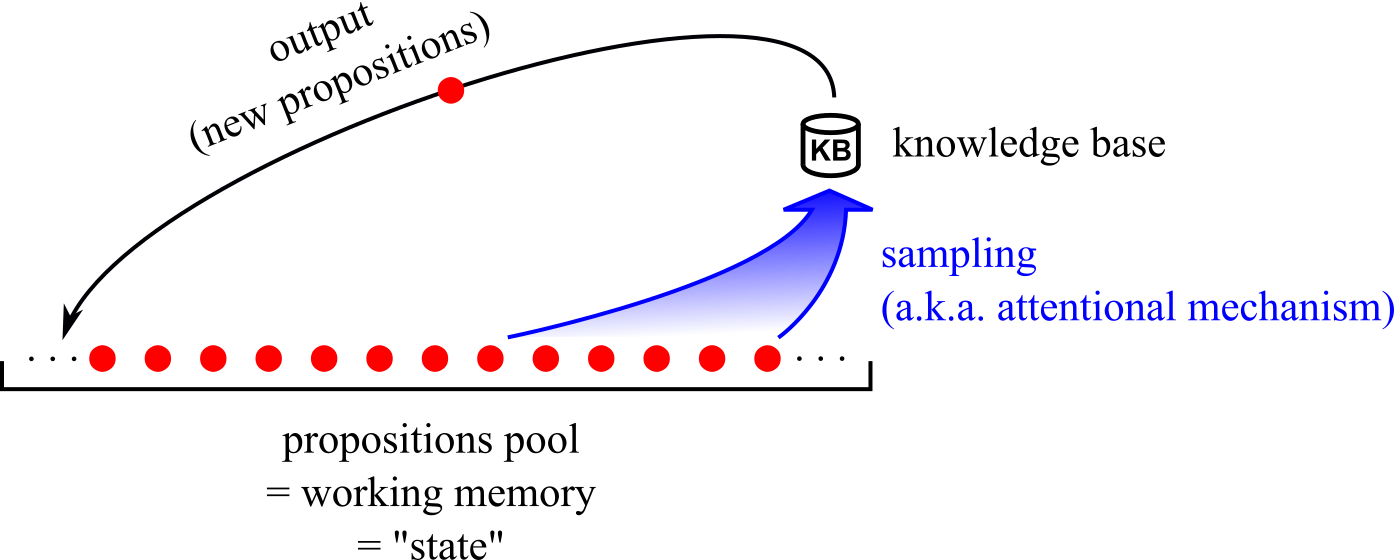
\includegraphics[scale=0.6]{classical-AI-architecture.png}}}
\end{equation}
\begin{itemize}
	\item \cc{working memory 是一些命题的集合}
	{working memory is a set of propositions}
	\item \cc{KB 代表系统的所有\textbf{知识}的总和}
	{KB stores the totality of knowledge in the system}
	\item \cc{attention 就是现在深度学习中很火的概念,但在这架构下,它和 cognitive science 的「注意力」是完全一样的}
	{The idea of attention is a current hot topic in deep learning.  In our architecture, attention coincides with the same notion in cognitive science.}
\end{itemize}
\cc{
关於这方面的理论可以在任何经典 AI 教科书找到。}{
The theoretical background can be found in any classical AI textbook.	
}

\cc{
我提出的 architecture 是用 deep neural network 代替 $\KB$ 的工作:}{
The architecture I propose is to use a deep neural network to replace the work of $\KB$:
}
\begin{equation}
\vcenter{\hbox{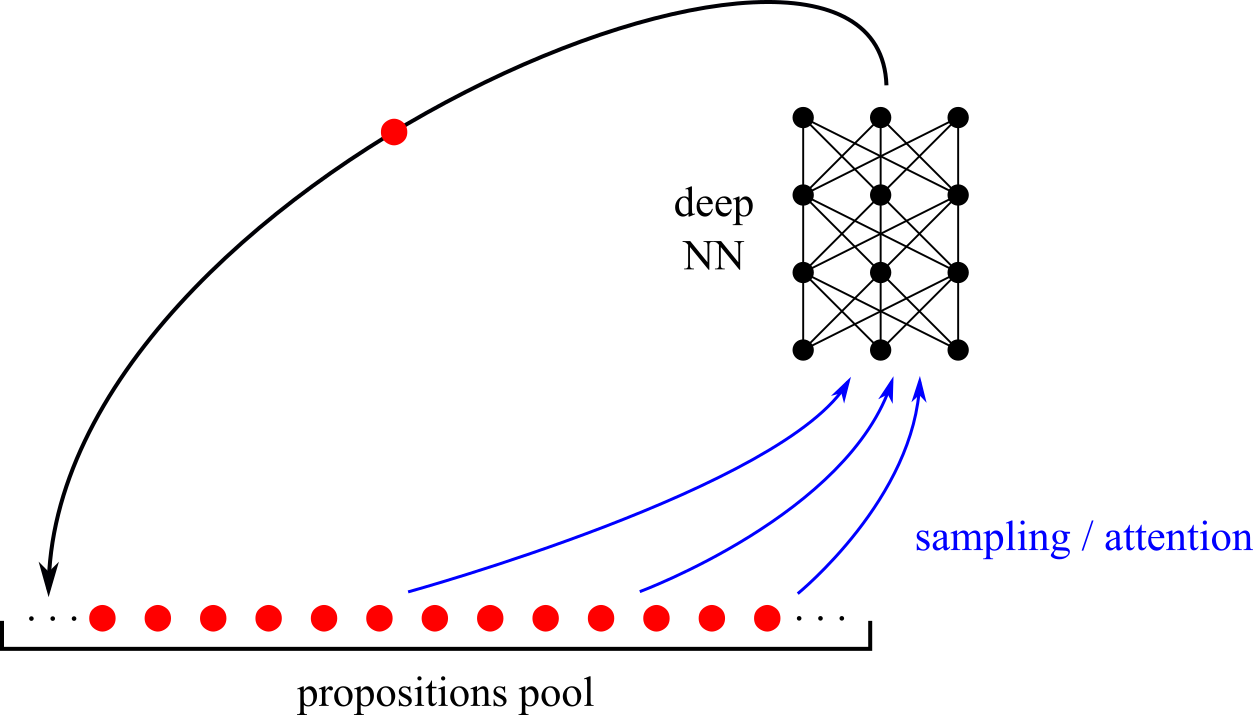
\includegraphics[scale=0.6]{simple-architecture.png}}}
\end{equation}
\cc{
因为经典 AI 的「死穴」是 learning 太慢,它用的方法是 inductive logic learning,这领域的著名研究者包括 Stephen Muggleton, Luc de Raedt, Ivan Bratko, A. Srinivasan 等人(抱歉有很多遗漏),但基本上没有重大突破,导致经典 AI 的停滞。
}{
The Achilles' heel of classical logic-based AI is that \uline{learning is too slow}, it uses \textbf{inductive logic learning}, the prominant researchers in this area include Stephen Muggleton, Luc de Raedt, Ivan Bratko, A. Srinivasan, and others (sorry that I am just recalling from memory).  The field lacked significant breakthroughs, that led to the ``winter'' of logic-based AI.
}

\subsubsection{\cc{神经网络为什么 powerful?}{Why are neural networks so powerful?}}

\cc{
Deep learning 是现时最强的机器学习方法,理由是因为: 它的输入和输出可以看成是 $\mathbb{R}^n \rightarrow \mathbb{R}^n$ 也可以看成是 二元化了的 $\{0,1\}^n \rightarrow \{0,1\}^n$ 亦即是 $n$-dimension hypercube 的顶点(共 $2^n$ 个)。  神经网络里 \textbf{参数} 的个数是:}{
Deep learning is the most powerful machine learning technique nowadays.  Its strength lies in the fact that a deep neural network can realize a huge family of functions using a relatively small number of parameters.  Assume that the network maps from $\mathbb{R}^n \rightarrow \mathbb{R}^n$, or the binarized form $\{0,1\}^n \rightarrow \{0,1\}^n$, which are the vertices of the $n$-dimension \textbf{hypercube}.  The number of parameters in the neural network is:
}
\begin{equation}
L \; n^2 \nonumber
\end{equation}
\cc{
其中 $L$ 是层数,假设每层都是 square matrix, fully connected.  但在输入和输出空间之间的函数的个数是:}{
where $L$ = \#(layers), assuming every layer is a square matrix, fully connected.  Whereas, the number of functions that exists between the input and output spaces is:
}
\begin{equation}
2^n \rightarrow 2^n = {(2^n)}^{2^n}
\end{equation}
\cc{
这在计算机科学里基本上就是「无限」。  换句话说,神经网络用相对地很少的参数,定义了一个函数家族,后者的数量是 \textbf{指数级} 的。 深度网络之所以能够这样,是因为随著层数的增加,整体函数的形状复杂性呈指数式上升(这复杂性可以用某种 topological degree 例如  Leray-Schauder degree 来描述)。 深度学习是现时唯一有这种特性的学习机器。}{
This is essentially ``infinity'' in computer science.  The number of functions grows exponentially, but a deep neural network can handle them because, as the number of layers grows, the possible shapes of the network function also increases exponentially (the complexity of shapes can be measured by a ``topological degree'' such as the Leray-Schauder degree).  Deep learning is the only learning machine with this property.
}

\cc{
有了问题的良好定义 (from classical AI),也有了武器,那么问题是必然可以解决的,只差在有人要将二者结合起来。  本文提出一个尝试。 }{
Now that we have a well-defined function, and we have the weapon, the problem's solution should not be far away.  Someone just needs to combine the two aspects.  Here we propose one such attempt.
}

\subsubsection{\cc{逻辑的命题结构}{The propositional structure in logic}}

\cc{
在这 architecture 中,deep NN 的输入是一些命题 (encoded as vectors),输出是一些新的命题(逻辑推导的结论)。 
}{
In this architecture, the deep NN inputs a set of propositions (encoded as vectors), and outputs some new propositions (the result of logical inference).
}

\cc{
这 architecture 的重点是它应用了逻辑中的 \textbf{propositional structure}。 在哲学逻辑中,\textbf{命题} 的概念是非常基本的: \uline{命题就是能赋予真假值的东西}。  如果连命题结构也不接受,则整个经典逻辑也不用玩了。  }{
The special point of this architecture is that it respects the propositional structure of logic.  In philosophical logic, the notion of the proposition is of central importance.  Basically, \uline{a proposition is an entity that we can assign true or false}.  If we abandon even this notion, there wouldn't be much left of classical logic.
}

\cc{
命题结构的特点是 \textbf{可交互性} (commutativity):}{
The essential property of propositions is their \textbf{commutativity}:
}
\begin{equation}
A \wedge B = B \wedge A
\end{equation}
\cc{
所以在 propositions pool 里,可以将命题任意排序,\uline{the order in which they are presented to the deep NN is unimportant}.  我较早前提出了 symmetric neural network, 即 $F(a, b) = F(b, a)$ 的一种函数,但现在弃用这一方法,理由是因为 rule matching 是更重要的樽颈问题.....}{
which is why, in the propositions pool, we can arrange the order of propositions arbitrarily, and \uline{the order in which they are presented to the deep NN is unimportant}.  I have previously proposed a kind of \textbf{symmetric NN} of the functional form $F(a, b) = F(b, a)$, but I have abandoned this idea for the reason explained in the next section....
}

\section{Rule matching}

\subsubsection{\cc{「以 facts 找 rules」}{``Finding rules with facts''}}

\cc{
在经典 AI 里有个很重要的问题: 已知一些 facts,如何在 $\KB$ 中找到适合 apply 的 rules?  这个问题在 1970's 年代已有解答,即 Rete algorithm(拉丁文,\textit{rete} 的意思是「网状」)。  Rete 算法的重点是: 「\uline{以 facts 找 rules,而不是用 rules 找 facts}」,理由很简单: 因为在 working memory 中 facts 的个数不算很大,但在 $\KB$ 中 rules 的个数是海量的。 细节从略。}{
In classical logic-based AI there used to be a critical problem:  given some facts, how to find the applicable rules in the $\KB$?  This is solved in the 1970s by the Rete algorithm (\textit{rete} in Latin means something like ``threads'').  The main idea in Rete is:  searching rules by facts, instead of searching facts by rules.  The reason is simple:  the number of facts in working memory is relatively small, but the number of rules in $\KB$ is enormous.
}

\cc{
后来,Rete 被应用到 SOAR architecture,这是一个著名的 rules engine 兼 cognitive architecture,在 Carnegie-Mellon 大学发展的。 但当然,它仍未能做到 strong AI,因为先前已经说过,logic AI 最严重的樽颈是 learning。 }{
Later, Rete is employed in the SOAR architecture, a famous cognitive architecture cum rule engine, developed in Carnegie-Mellon University.  Of course, SOAR did not achieve AGI, as I explained earlier, the Achilles' heel is in learning.
}

\cc{
在我们的 architecture 里,learning 交给 deep NN 做,但 rule matching 仍然是一个很费时的动作。  虽然说 recurrent neural network 有 ``unreasonable effectiveness'',但既然 rule matching 这动作的结构已知,似乎不应该浪费资源让 RNN 「由零开始」学习它,否则学习太慢仍会失败。 }{
In our architecture, learning is delegated to the deep NN, but rule matching is still a very time-consuming operation.  Even if one believes in the ``unreasonable effectiveness'' of recurrent neural networks, there is a strong reason to implement rule matching explicitly, instead of letting the RNN learn it from scratch, which could still be too slow.
}

\cc{
我提出的解决方法,其实和 Rete 的思路是一样的: 以 facts 找 rules。 举例来说,有这样一条 rule:}{
The solution I propose, is along the same thinking as Rete:  searching rules by facts.  For example, we may have the following rule:
}
\begin{equation}
\label{eqn:rule-example}
A \wedge B \wedge C \rightarrow D
\end{equation}
\cc{
其中 $A, B, C, D$ 是命题。  解决办法是反过来将 $A \wedge B \wedge C$ 这个 conjunction 用一个 \textbf{点} 表示,而命题 $A, B, C$ 用一些 regions(区域)表示。 如果 region $A$ 包含 \textbullet,表示 $A$ 有份参与在这个 conjunction 里:}{
where $A, B, C, D$ are propositions.  The trick is to ``invert'' the conjunction $A \wedge B \wedge C$ by representing it as a \textbf{point}, whereas the propositions $A, B, C$ are represented by some \textbf{regions}.  If the region $A$ includes \textbullet, that means $A$ participates in this conjunction:
}
\begin{equation}
\vcenter{\hbox{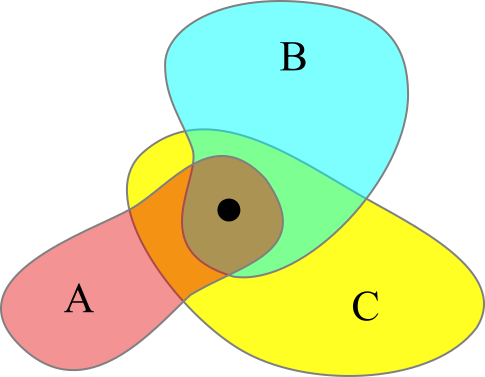
\includegraphics[scale=0.6]{conjunction-vertex.png}}}
\end{equation}
\cc{
这样做的用意是: 每个 proposition 是一个 region 也可以看成是一个 characteristic function,它输入某 \textbf{点} 的位置,输出 true 或 false 表示这点属不属於该 region。  换句话说它就像一个 ``agent'',输入 conjunction,它回答它自己有没有参与这 conjunction,换句话说就是「以 fact 找 rule」。}{
The intention is:  each proposition is a region which can also be regarded as \textbf{characteristic function}:  it inputs a certain \textbf{point} location, and outputs true or false depending if that point belongs to the region.  In other words it is like an ``agent'', input a conjunction, it outputs if it participates in this particular conjunction.  In other words, it is ``searching rules by facts''.
}

\cc{
具体做法是这样的: 需要很多的点代表 conjunctions,不妨令 hypercube 的 $2^n$ 个 vertices 做这些点。 因为每个形如 (\ref{eqn:rule-example}) 的 rule 都有一个 conjunction,所以 这些点的个数就是 $\KB$ 里 rules 的 \textbf{总数}。 换句话说,deep NN 的作用是: 已找到 rule,apply 那 rule。 Rule matching 的工作分拆出来做,NN 只是学习和储存 $\KB$ 的 rules。 }{
Actual implementation is as follows:  As we need many points to represent conjunctions, we could take the $2^n$ vertices of the hypercube.  And as each rule of the form (\ref{eqn:rule-example}) is associated with one conjunction, the number of vertices of the hypercube is the total number of rules in $\KB$.  In other words, the job of the deep NN is just to learn, store and \textbf{apply} the rules that have been found.  The rule matching task is separated out.
}

\cc{
Architecture 变成这样(但仍有问题):}{
Now the architecture becomes like this (but it still has a problem):
}
\begin{equation}
\vcenter{\hbox{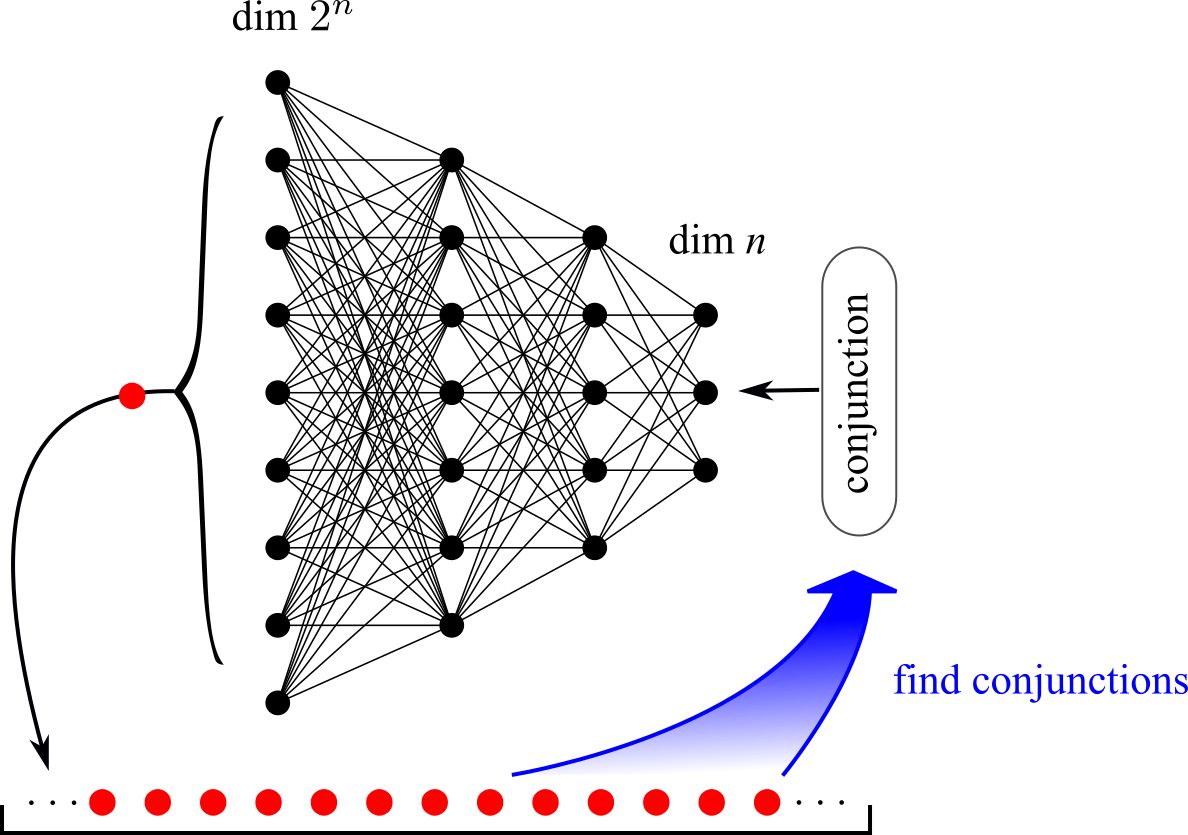
\includegraphics[scale=0.6]{conjunction-architecture.png}}}
\end{equation}
\cc{
NN 的输入端是 hypercube 的某个 vertex,这 vertex 代表某 conjunction。 换句话说,输入是一个 binary vector of dimension $n$.  输出是一个 proposition,而根据我们的设定,proposition 就是 hypercube 的所有 vertices 的某 subset。 换句话说,输出 $\in 2^{2^n}$。 如果输出也是一支 binary vector,则其长度是 $2^n$。  当 $n > O(10)$ 时,变得不切实际。  举例来说,你或许会相信人类智能的 $\KB$ size $\approx 2^{100}$ 至 $2^{1000}$ 或以上,但如果是 $2^{20} = 1048576$ 则似乎太少了。  换句话说,NN 输出的 proposition representation 需要 \textbf{压缩}。}{
The NN recieves its input as a single vertex of the hypercube, which represents a conjunction.  In other words, the input is a binary vector of dimension $n$.  Output is a proposition;  and from our setup, a proposition is a \textbf{subset} of vertices of the hypercube.  That is to say, output $\in 2^{2^n}$.  If this output is also represented as a binary vector, its length would be $2^n$.  Clearly, when $n > O(10)$ this becomes rather infeasible.  For instance, you may believe that human intelligence requires a $\KB$ of size $\approx 2^{100}$ to $2^{1000}$ or even more, but if it is $2^{20} = 1048576$ then it might be too small.  Therefore, the NN's output representation of the proposition needs to be \textbf{compressed}.
}

\cc{
压缩的意思是: 将长度为 $2^n$ 的 vector,用较短的 vector 代表。  这 encoding 可以是一个 $2^n \rightarrow \vect{2}$ 的近似函数(输入某个 vertex = conjunction,输出 yes / no)\footnote{实际上,每个 conjunction 的子命题个数 $k$ 不同,所以要使用 $2^n \rightarrow \mathbb{R}$ 或 $2^n \rightarrow [0,1]$ 的形式。 而且,要避免同一个命题被 counted twice。},例如:}{
Compression means to encode the vector of length $2^n$ by a shorter vector.  This encoding could be an approximating function $f: 2^n \rightarrow \vect{2}$ (input is a certain vertex = conjunction, output = yes / no) \footnote{In practice, a conjunction may have a variable number $k$ of conjuncts, so we may need to use $2^n \rightarrow \mathbb{R}$ or $2^n \rightarrow [0,1]$.  Also, we need to avoid counting a proposition twice in the proposition pool.}, for example:
}
\begin{itemize}
	\item \cc{输出一串神经网络的 weights,这些 weights 再建立一个 \textbf{小神经网络} $F: 2^n \rightarrow \vect{2}$ \\}
	{NN outputs a series of weights, which constructs a \textbf{small neural network} $F: 2^n \rightarrow \vect{2}$ \\}
	In other words, each proposition is a micro-neural network.
	\item \cc{用}{use} multi-variate discrete Fourier transform,truncate low-energy terms
\end{itemize}
\cc{
这压缩的步骤很麻烦,第一种方法基本上就是「大 NN 输出小 NN」,其可行性未经证实。  需要压缩的原因来自: proposition representation 的长度太长。  解决的办法或许是将 proposition representation 的复杂性的一部分转移到 conjunction 的 representation 中去。 但这样做有没有用? 它只是将输出 representation 的复杂性转移到输入 representation 的复杂性。 暂时想到这里。 \footnote{这个压缩的问题,在我提出的另一个 AGI architecture 里也遇到过,当时的目标是做到 Cartesian closed category 的 $X^X \cong X$.  方法是让神经网络的输出直接写入神经网络自己的 weights。 但 weights 的个数显然 $\gg$ 于输出向量的维数,所以在那情况下亦需要压缩。 我的感觉是,这压缩问题显示了 AGI 问题的樽颈所在。}}{
This compression step is rather troublesome.  The first method is essentially to ``use big NN to output small NNs'', whose workability remains to be proven.  The need for compression comes from the too-long length of the proposition representation.  One idea is to transfer the complexity of the proposition representation to the conjunction representation.  But is this useful?  We'd just be transferring the complexity from the output representation to the input representation of the same NN.  This is my thinking so far.  \footnote{About this compression problem, I have previously encountered it in a similar form, while designing a different AGI architecture.  Then, my goal was to achieve $X^X \cong X$ of a Cartesian closed category.  My solution is to let the NN write to its own weights.  But the number of weights in an NN is clearly $\gg$ the dimension of the output vector, so we needed compression in that situation as well.  My feeling is that the need for compression is an indication of the AGI bottleneck.}
}

\subsubsection{Stochastic local search for matching}

\cc{
馀下一个细节: 根据以上的设计,给出一串命题,如何找成立的 conjunction(s)?  算法的灵感来自 GSAT 和 WalkSAT,SAT 就是命题逻辑的 satisfiability,著名的 NP-complete 问题。 SAT 和我们的 matching 问题非常相似,可能是同构的(?)}{
One remaining detail:  according to the above design, given a set of propositions, how do we find the satisfying conjunctions?  An inspiration comes from the GSAT and WalkSAT algorithms for propositional satisfiability, the famous NP-complete problem.  SAT is very similar to our problem, perhaps even isomorphic (?)
}

\cc{
GSAT 的 G 是 greedy 的意思,WalkSAT 是指 random walk。 实践证明,greedy + stochastic search 是对 SAT 问题非常有效的 heuristics.}{
The G in GSAT means greedy, whereas WalkSAT refers to random walk.  It has been proven in practice that greedy + stochastic search are highly effective heuristics for solving SAT.
}

\cc{
如前所述,每个 proposition 是一个由 vertex $\rightarrow$ true / false 的 micro-function。 可以将这输出固定在 true 位置,用 \textbf{反向传播} 得出一些 satisfying vertex 的例子(不是唯一的)。  用 list 记住这些 vertices.}{
As mentioned earlier, each proposition is a micro-function $f:$ vertex $\rightarrow$ true / false.  We can \textbf{clamp} the output value to true, and use \textbf{backward propagation} to obtain some instances of satisfying vertices (these are not unique).  Use a list to store these vertices.
}

\cc{
然后或者可以用 genetic algorithm 进化这些 vertices,直到找到有 satisfied conjunction.
}{
And then perhaps we can use a \textbf{genetic algorithm} to evolve these vertices until we find a satisfied conjunction.	
}

\begin{comment}
\begin{itemize}
	\item Randomly initialize an assignment = 某个 vertex = 某 conjunction
	\item Run every proposition (micro-NN) forward, find which ones are ``ON'' \\
		  (If output value > 0, it means the proposition ``covers'' the conjunction)
	\item If the sum of covers $>$ threshold, that conjunction is satisfied
	\item Else, try next conjunction by ``flipping'' \\
		  (Flipping means changing the coordinate of a vertex from 0 to 1 or \textit{vice versa}) \\
\end{itemize}
\end{comment}

\section{Learning}

\cc{
学习算法很简单,基本上是 deep reinforcement learning,根据 Bellman update。 训练时需要有智能的 teacher 或 training data 给予奖励或惩罚。  这方面已经是一个有深入研究的课题,例如 UC Berkeley 公开了《深度强化学习》的网上课程。}{
Learning is simply the application of \textbf{deep reinforcement learning}, via the \textbf{Bellman update}.  Training requires rewards and punishment information from a teacher or training data set.  This is a well-researched topic, for example there is an online course on DRL from UC Berkeley.
}

\cc{
Credit assignment 问题:  奖与罚并不是做每一个逻辑推导即时获得的,它可能出现在一连串的 inference chain 之后,这 inference chain 其实就是 强化学习里面的 \textbf{eligibility trace} 概念。  换句话说,整条 \textbf{逻辑推导链},同时获得奖励和惩罚(也就是将那些「有责任的」 weights 增强/减弱)。  All the weights in the NN can be re-normalized periodically.}{
The \textbf{credit assignment} problem:  rewards and punishment is not instantly received after a single inference step, but may appear after a long \textbf{inference chain}.  This inference chain plays the same role as the \textbf{eligibility trace} in reinforcement learning.  In other words, the entire chain needs to be rewarded or punished during learning (in other words, increase or decrease the weights that were \textbf{responsible} in the inference chain).  All the weights in the NN can be re-normalized periodically.
}

\subsubsection{A note about natural language}

\cc{
将 internal representation 转换成自然语言,只需额外的 logical inference,但在学习 internal representation 和 知识 的同时,要学习这 language generation 的能力可谓难上加难。  因为奖与罚的时候并不知道是内在知识有问题还是语言的表达有问题。 所以建议在开始训练时不要同时学习知识和语言表达。  然而,人类在讲述自己没有信心的内容时,也会有「结结巴巴」的现象,这似乎表示,内在知识和语言表达的 inference chains 同时受奖与罚是「正常」的 $\smiley$}{
To generate natural language from internal representations, we only need additional logical inference.  However, to learn language generation while learning the internal representation and knowledge at the same time might be too difficult, so we would advice against trying these as first experiments.  However, even for humans, talking about things that one is not confident about, often results in stammering and other speech disturbances.  This may be evidence that rewarding / punishing the inference chains for language and for real knowledge at the same time, may be ``normal'' $\smiley$
}

\section{Conclusion}

\cc{
目前最不满意的地方是 proposition representation 所需的压缩。  因为命题是一些 micro-神经网络,改变一个 weight 的作用很微小,有 vanishing gradient 的忧虑。  但笔者亦庆幸越来越看到 AGI 接近实践的地步。}{
One thing we are not satisfied with is the need for compression of the proposition representation.  Representing a proposition as a micro-NN, changing its weights may have very small and indirect effects, thus the vanishing gradient is a worry.  But I am glad to see the goal of AGI getting more and more achievable.
}

\begin{comment}
\section{Deep RNN}

The equation for one layer of RNN is:
\begin{equation}
x_{n+1} = \sigmoid (W x + H x)
\end{equation}
\end{comment}

\section*{Acknowledgements}

\cc{
将神经网络和 von Neumann architecture style 的程式混合,这种做法虽然缺乏美感但可能是很有效的。 我在读 Andrew Ng \textit{et al} 提出的 recursive neural network(有别於 recurrent neural network)时看到这种例子。 }{
Mixing neural networks with von Neumann-style architecture programming, while biologically inelegant, may be highly effective.  I saw an example of this from Andrew Ng \textit{et al}'s paper on recursive neural networks (not to be confused with recurrent neural networks).
}

\bibliographystyle{unsrtnat} % or number or aaai ...
\bibliography{AGI-book}

\end{document}
